
\documentclass[11pt,a4paper]{article}

\usepackage[T1]{fontenc}
\usepackage[utf8]{inputenc}
\usepackage[dutch]{babel}
\usepackage{lmodern}
\usepackage{microtype}
\usepackage[a4paper,margin=2.1cm]{geometry}
\usepackage{amsmath,amssymb}
\usepackage{booktabs,array,tabularx}
\usepackage{enumitem}
\usepackage{xcolor}
\usepackage{tikz}
\usetikzlibrary{arrows.meta,decorations.pathmorphing,positioning,calc,patterns}

\definecolor{notegray}{RGB}{245,245,245}
\definecolor{uncertain}{RGB}{145,70,0}
\definecolor{inkblue}{RGB}{28,78,150}
\definecolor{inkred}{RGB}{190,45,45}
\definecolor{inkgreen}{RGB}{35,135,75}

\newcommand{\uncertain}[1]{\textcolor{uncertain}{\textit{[onzeker: #1]}}}
\newcommand{\literalnote}[1]{%
  \begin{center}
  \fcolorbox{black!35}{notegray}{%
    \begin{minipage}{0.92\linewidth}
      #1
    \end{minipage}}
  \end{center}
}
\newcommand{\photon}[3]{%
  \draw[#3,decorate,decoration={snake,amplitude=2pt,segment length=6pt},->,thick]
    (#1)--(#2);
}
\newcommand{\atom}[4]{%
  \draw[inkblue,thick] (#1,#2) circle (#3);
  \fill[inkred!70] (#1,#2) circle (0.12);
  \fill[inkblue] ({#1+#3*cos(#4)},{#2+#3*sin(#4)}) circle (0.07);
}

\title{\textbf{Kwantum Natuurkunde}\\
\large LaTeX-transcriptie van PDF-pagina's 6--10}
\author{}
\date{}

\begin{document}
\maketitle

\noindent
Deze transcriptie is gebaseerd op visuele inspectie van de oorspronkelijke
scans op hoge resolutie. De spelling en formulering zijn zoveel mogelijk
letterlijk behouden. Onduidelijke passages zijn gemarkeerd met
\uncertain{tekst}. De natuurkundige inhoud is niet stilzwijgend gecorrigeerd;
waar nuttig wordt een gangbare notatie afzonderlijk genoemd. Schematische
tekeningen zijn in TikZ gereconstrueerd.

% --------------------------------------------------------------------------
\section*{PDF-pagina 6 --- golf-deeltjesdualiteit}

\subsection*{Linker notitiepagina: ``Golf/deeltjes: Dualiteit''}

\begin{center}
{\Large \textbf{Twee-spletenexperiment}}
\end{center}

\begin{center}
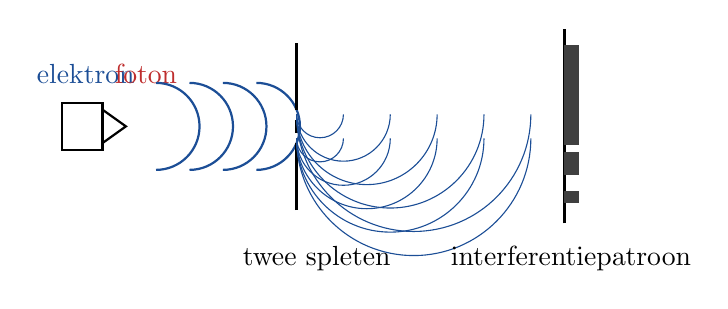
\begin{tikzpicture}[>=Latex,x=0.85cm,y=0.85cm]
  % Bron
  \draw[thick] (-5.6,-0.35) rectangle (-5.0,0.35);
  \draw[thick] (-5.0,-0.25)--(-4.65,0)--(-5.0,0.25);
  \node[inkblue,above] at (-5.25,0.5) {elektron};
  \node[inkred,above] at (-4.35,0.5) {foton};

  % Inkomende golffronten
  \foreach \x in {-4.2,-3.7,-3.2,-2.7}
    \draw[inkblue,thick] (\x,-0.65) arc (-90:90:0.65);

  % Dubbele spleet
  \draw[very thick] (-2.1,-1.25)--(-2.1,-0.25);
  \draw[very thick] (-2.1,0.25)--(-2.1,1.25);
  \draw[very thick] (-2.1,-0.1)--(-2.1,0.1);

  % Uitgaande golven
  \foreach \r in {0.35,0.7,1.05,1.4,1.75}
  {
    \draw[inkblue] (-2.1,0.18) arc (180:360:\r);
    \draw[inkblue] (-2.1,-0.18) arc (180:360:\r);
  }

  % Scherm / interferentie
  \draw[very thick] (1.9,-1.45)--(1.9,1.45);
  \foreach \y/\h in {-1.15/0.18,-0.72/0.34,-0.28/0.55,0.15/0.75,0.58/0.42,1.0/0.22}
    \fill[black!75] (1.9,\y) rectangle +(0.22,\h);
  \node[below] at (-1.8,-1.65) {twee spleten};
  \node[below] at (2.0,-1.65) {interferentiepatroon};
\end{tikzpicture}
\end{center}

De twee getekende superposities zijn schematisch:

\begin{align*}
\text{gelijke fase:}\qquad
\sin(\omega t)+\sin(\omega t)
  &=2\sin(\omega t),\\
\text{tegengestelde fase:}\qquad
\sin(\omega t)+\sin(\omega t+\pi)
  &=0.
\end{align*}

\begin{center}
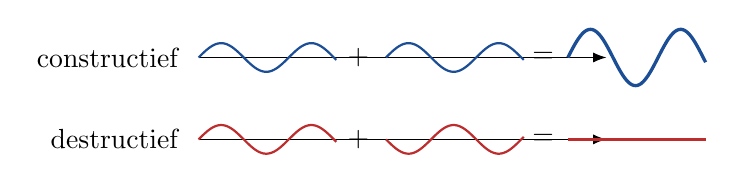
\begin{tikzpicture}[>=Latex,x=0.7cm,y=0.65cm]
  \node[anchor=east] at (-0.2,1.2) {constructief};
  \draw[->] (0,1.2)--(7.4,1.2);
  \draw[inkblue,thick,domain=0:2.5,samples=80]
    plot(\x,{1.2+0.28*sin(220*\x)});
  \node at (2.9,1.2) {$+$};
  \draw[inkblue,thick,domain=3.4:5.9,samples=80]
    plot(\x,{1.2+0.28*sin(220*(\x-3.4))});
  \node at (6.25,1.2) {$=$};
  \draw[inkblue,very thick,domain=6.7:9.2,samples=80]
    plot(\x,{1.2+0.55*sin(220*(\x-6.7))});

  \node[anchor=east] at (-0.2,-0.4) {destructief};
  \draw[->] (0,-0.4)--(7.4,-0.4);
  \draw[inkred,thick,domain=0:2.5,samples=80]
    plot(\x,{-0.4+0.28*sin(220*\x)});
  \node at (2.9,-0.4) {$+$};
  \draw[inkred,thick,domain=3.4:5.9,samples=80]
    plot(\x,{-0.4-0.28*sin(220*(\x-3.4))});
  \node at (6.25,-0.4) {$=$};
  \draw[inkred,very thick] (6.7,-0.4)--(9.2,-0.4);
\end{tikzpicture}
\end{center}

In de marge staat: ``3:27:00, deel 2''.

\literalnote{%
Vanwege het feit dat de massa van de foton en elektron gelijk
\uncertain{blijven tijdens de excitatie}, is het enige wat de snelheid kan
minderen de magnetische tegencomponenten. De enige kracht die groot genoeg
kan worden is de gravitomagnetische \uncertain{component/kracht; zin loopt af
aan de paginarand}.}

\subsection*{Rechter notitiepagina: ``Foton vs. Elektron''}

Boven de elektron-schets staat ``Magnetische component''. De foton-schets
wordt als een oscillerende lading getekend; de elektron-schets als een
combinatie van een elektrische en een magnetische oriëntatie.

\begin{center}
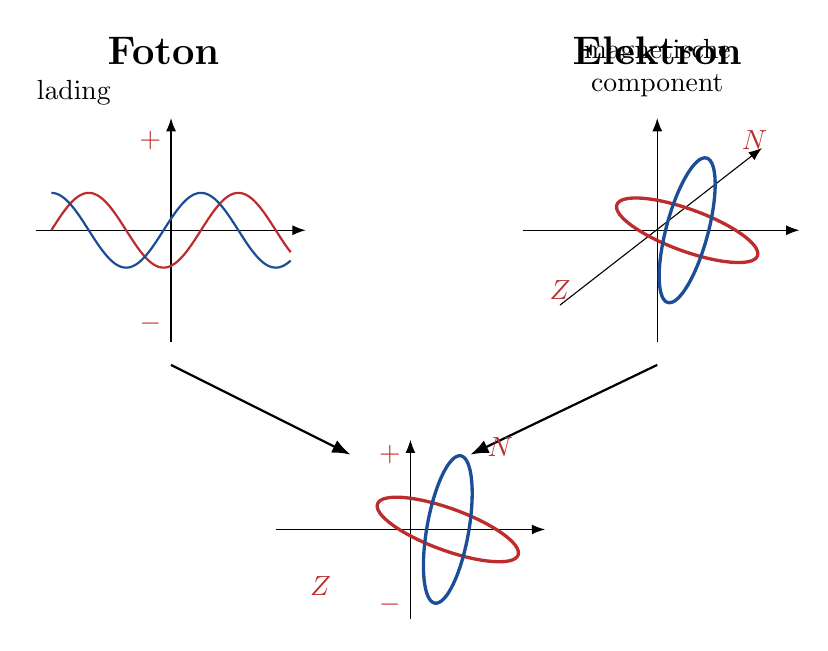
\begin{tikzpicture}[>=Latex,scale=0.95]
  \node[font=\Large\bfseries] at (-3.3,3.4) {Foton};
  \node[font=\Large\bfseries] at (3.3,3.4) {Elektron};

  % Photon axis and wave
  \draw[->] (-5.0,1.0)--(-1.4,1.0);
  \draw[->] (-3.2,-0.5)--(-3.2,2.5);
  \node[inkred,left] at (-3.2,2.2) {$+$};
  \node[inkred,left] at (-3.2,-0.25) {$-$};
  \draw[inkred,thick,domain=-4.8:-1.6,samples=100]
    plot(\x,{1.0+0.5*sin(180*(\x+4.8))});
  \draw[inkblue,thick,domain=-4.8:-1.6,samples=100]
    plot(\x,{1.0+0.5*cos(180*(\x+4.8))});
  \node[above] at (-4.5,2.55) {lading};

  % Electron axes / loops
  \draw[->] (1.5,1.0)--(5.2,1.0);
  \draw[->] (3.3,-0.5)--(3.3,2.5);
  \draw[->] (2.0,0.0)--(4.7,2.1);
  \draw[inkred,very thick,rotate around={-20:(3.7,1.0)}]
    (3.7,1.0) ellipse (1.0 and 0.28);
  \draw[inkblue,very thick,rotate around={75:(3.7,1.0)}]
    (3.7,1.0) ellipse (1.0 and 0.28);
  \node[inkred] at (4.6,2.2) {$N$};
  \node[inkred] at (2.0,0.2) {$Z$};
  \node[above,align=center] at (3.3,2.65) {magnetische\\component};

  \draw[->,thick] (-3.2,-0.8)--(-0.8,-2.0);
  \draw[->,thick] (3.3,-0.8)--(0.8,-2.0);

  % Combined object
  \draw[->] (-1.8,-3.0)--(1.8,-3.0);
  \draw[->] (0,-4.2)--(0,-1.8);
  \draw[inkred,very thick,rotate around={-20:(0.5,-3.0)}]
    (0.5,-3.0) ellipse (1.0 and 0.28);
  \draw[inkblue,very thick,rotate around={80:(0.5,-3.0)}]
    (0.5,-3.0) ellipse (1.0 and 0.28);
  \node[inkred] at (1.2,-1.9) {$N$};
  \node[inkred] at (-1.2,-3.75) {$Z$};
  \node[inkred,left] at (0,-2.0) {$+$};
  \node[inkred,left] at (0,-4.0) {$-$};
\end{tikzpicture}
\end{center}

% --------------------------------------------------------------------------
\newpage
\section*{PDF-pagina 7 --- kwantumexcitatie}

\subsection*{Linker notitiepagina}

\begin{center}
{\Large \textbf{Kwantum Excitatie}}
\end{center}

\begin{center}
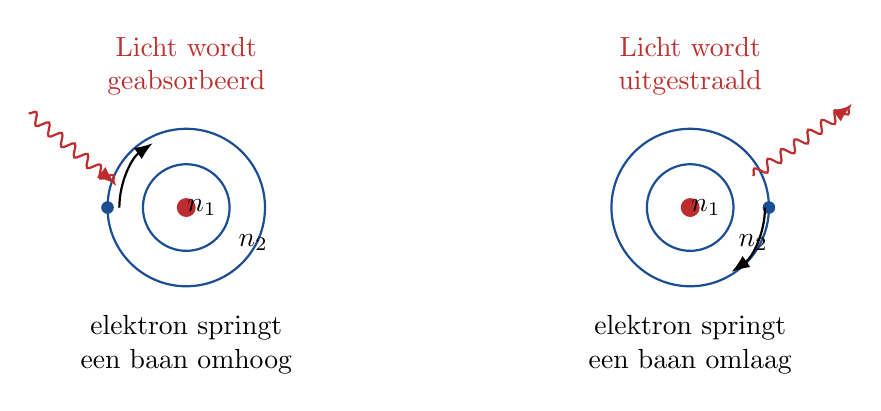
\begin{tikzpicture}[>=Latex,x=1cm,y=1cm]
  % absorption
  \node[inkred,align=center] at (-3.2,3.2) {Licht wordt\\geabsorbeerd};
  \draw[inkblue,thick] (-3.2,1.4) circle (0.55);
  \draw[inkblue,thick] (-3.2,1.4) circle (1.0);
  \fill[inkred] (-3.2,1.4) circle (0.12);
  \fill[inkblue] (-4.2,1.4) circle (0.08);
  \photon{-5.2,2.6}{-4.1,1.7}{inkred}
  \draw[->,thick] (-4.05,1.4) arc (180:125:1.0);
  \node[below,align=center] at (-3.2,0.15)
    {elektron springt\\een baan omhoog};

  % emission
  \node[inkred,align=center] at (3.2,3.2) {Licht wordt\\uitgestraald};
  \draw[inkblue,thick] (3.2,1.4) circle (0.55);
  \draw[inkblue,thick] (3.2,1.4) circle (1.0);
  \fill[inkred] (3.2,1.4) circle (0.12);
  \fill[inkblue] (4.2,1.4) circle (0.08);
  \draw[->,thick] (4.15,1.4) arc (0:-55:1.0);
  \photon{4.0,1.8}{5.25,2.7}{inkred}
  \node[below,align=center] at (3.2,0.15)
    {elektron springt\\een baan omlaag};

  % orbit labels
  \node at (-3.0,1.4) {$n_1$};
  \node at (-2.35,0.95) {$n_2$};
  \node at (3.4,1.4) {$n_1$};
  \node at (4.0,0.95) {$n_2$};
\end{tikzpicture}
\end{center}

De onderste reeks tekeningen toont hetzelfde proces vanuit een andere
oriëntatie: een invallend foton vergroot de baan van het elektron van
$n_2$ naar $n_3$.

\begin{center}
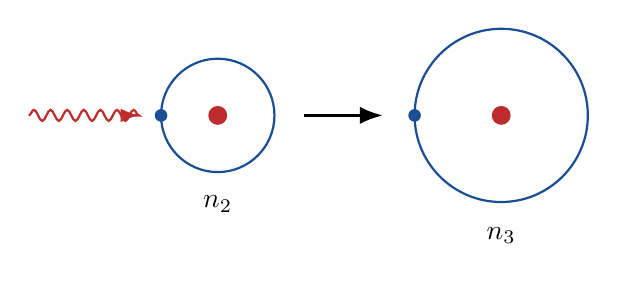
\begin{tikzpicture}[>=Latex,x=1cm,y=1cm]
  \photon{-5,0}{-3.6,0}{inkred}
  \draw[inkblue,thick] (-2.6,0) circle (0.72);
  \fill[inkred] (-2.6,0) circle (0.12);
  \fill[inkblue] (-3.32,0) circle (0.08);
  \node[below] at (-2.6,-0.9) {$n_2$};

  \draw[->,very thick] (-1.5,0)--(-0.5,0);

  \draw[inkblue,thick] (1.0,0) circle (1.10);
  \fill[inkred] (1.0,0) circle (0.12);
  \fill[inkblue] (-0.1,0) circle (0.08);
  \node[below] at (1.0,-1.3) {$n_3$};
\end{tikzpicture}
\end{center}

\subsection*{Rechter notitiepagina: ``Waterstof licht uitstralen''}

De pagina koppelt verschillende overgangen tussen $n_1$, $n_2$ en $n_3$ aan
verschillende kleuren licht.

\begin{center}
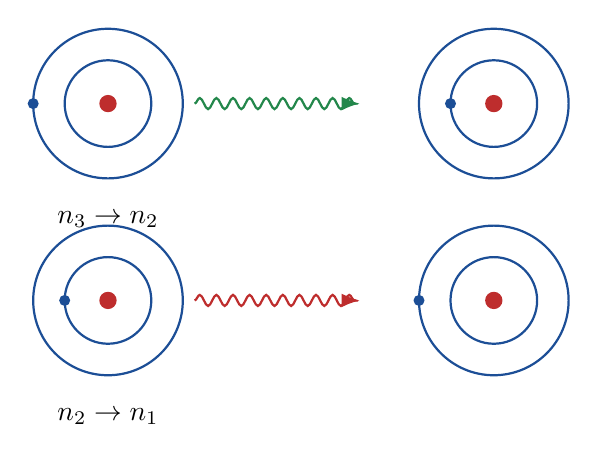
\begin{tikzpicture}[>=Latex,x=1cm,y=1cm]
  % top transition
  \draw[inkblue,thick] (-3.6,2.3) circle (0.55);
  \draw[inkblue,thick] (-3.6,2.3) circle (0.95);
  \fill[inkred] (-3.6,2.3) circle (0.11);
  \fill[inkblue] (-4.55,2.3) circle (0.07);
  \photon{-2.5,2.3}{-0.4,2.3}{inkgreen}
  \draw[inkblue,thick] (1.3,2.3) circle (0.55);
  \draw[inkblue,thick] (1.3,2.3) circle (0.95);
  \fill[inkred] (1.3,2.3) circle (0.11);
  \fill[inkblue] (0.75,2.3) circle (0.07);
  \node[below] at (-3.6,1.05) {$n_3\rightarrow n_2$};

  % second transition
  \draw[inkblue,thick] (-3.6,-0.2) circle (0.55);
  \draw[inkblue,thick] (-3.6,-0.2) circle (0.95);
  \fill[inkred] (-3.6,-0.2) circle (0.11);
  \fill[inkblue] (-4.15,-0.2) circle (0.07);
  \photon{-2.5,-0.2}{-0.4,-0.2}{inkred}
  \draw[inkblue,thick] (1.3,-0.2) circle (0.55);
  \draw[inkblue,thick] (1.3,-0.2) circle (0.95);
  \fill[inkred] (1.3,-0.2) circle (0.11);
  \fill[inkblue] (0.35,-0.2) circle (0.07);
  \node[below] at (-3.6,-1.45) {$n_2\rightarrow n_1$};
\end{tikzpicture}
\end{center}

Onderaan wordt invallend wit licht voorgesteld als meerdere kleuren die door
een waterstofatoom in afzonderlijke spectraallijnen worden uitgestraald:

\begin{center}
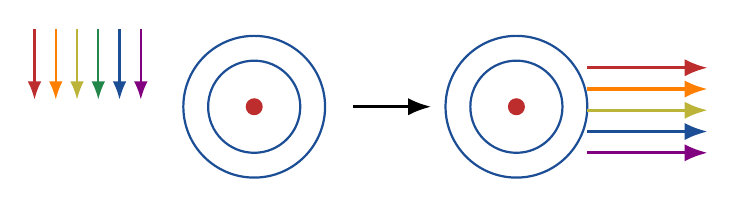
\begin{tikzpicture}[>=Latex,x=0.9cm,y=0.9cm]
  \foreach \x/\c in {-4.3/inkred,-4.0/orange,-3.7/yellow!70!black,-3.4/inkgreen,-3.1/inkblue,-2.8/violet}
    \draw[\c,thick,->] (\x,1.1)--(\x,0.1);

  \draw[inkblue,thick] (-1.2,0) circle (0.65);
  \draw[inkblue,thick] (-1.2,0) circle (1.0);
  \fill[inkred] (-1.2,0) circle (0.12);

  \draw[->,very thick] (0.2,0)--(1.3,0);

  \draw[inkblue,thick] (2.5,0) circle (0.65);
  \draw[inkblue,thick] (2.5,0) circle (1.0);
  \fill[inkred] (2.5,0) circle (0.12);
  \foreach \y/\c in {0.55/inkred,0.25/orange,-0.05/yellow!70!black,-0.35/inkblue,-0.65/violet}
    \draw[\c,very thick,->] (3.5,\y)--(5.2,\y);
\end{tikzpicture}
\end{center}

% --------------------------------------------------------------------------
\newpage
\section*{PDF-pagina 8 --- Dopplereffect}

\subsection*{Linker notitiepagina}

\begin{center}
{\Large \textbf{Dopler effect}}\\
\small ``cristiaan dopler 1842'' \hspace{1.5em} ``frequentie verschil''
\end{center}

De schets toont roodverschuiving bij een zich verwijderende bron en
blauwverschuiving bij een naderende bron.

\begin{center}
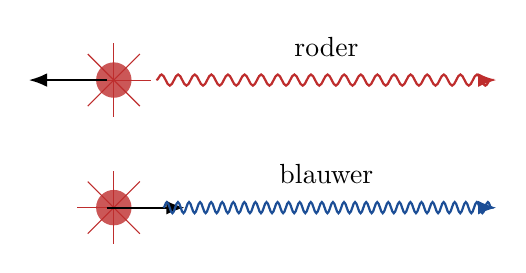
\begin{tikzpicture}[>=Latex,x=0.9cm,y=0.9cm]
  \fill[inkred!80] (-3,1.0) circle (0.25);
  \foreach \a in {0,45,...,315}
    \draw[inkred] (-3,1.0)--++(\a:0.52);
  \draw[->,thick] (-3.1,1.0)--(-4.2,1.0);
  \photon{-2.4,1.0}{2.4,1.0}{inkred}
  \node[above] at (0,1.2) {roder};

  \fill[inkred!80] (-3,-0.8) circle (0.25);
  \foreach \a in {0,45,...,315}
    \draw[inkred] (-3,-0.8)--++(\a:0.52);
  \draw[->,thick] (-3.1,-0.8)--(-2.0,-0.8);
  \draw[inkblue,decorate,decoration={snake,amplitude=2pt,segment length=4pt},->,thick]
    (-2.3,-0.8)--(2.4,-0.8);
  \node[above] at (0,-0.6) {blauwer};
\end{tikzpicture}
\end{center}

De bronformule staat genoteerd als:

$$
f_{\mathrm{eind}}
=
f_{\mathrm{bron}}
\left(
\frac{V}{V\pm V_{\mathrm{bron}}}
\right).
$$

De bijgeschreven definities zijn:

\begin{align*}
V &={}\text{snelheid},\\
V_b &={}\text{snelheid van de bron, na gelang van }f_{\mathrm{eind}},\\
f_b &={}\text{bronfrequentie},\\
f_{\mathrm{eind}} &={}\text{eindfrequentie}.
\end{align*}

\subsection*{Rechter notitiepagina}

Voor een bewegende waarnemer staat:

$$
f_{\mathrm{eind}}
=
f_{\mathrm{bron}}
\left(
1\pm\frac{V_w}{V}
\right),
$$

waarbij $V_w$ is omschreven als ``snelheid waarnemer''.

Voor een bewegende bron en waarnemer samen staat:

$$
f_{\mathrm{eind}}
=
f_{\mathrm{bron}}
\left(
\frac{V\pm V_w}{V-V_b}
\right).
$$

Onder ``Met Relativiteit'' staat letterlijk:

\begin{align*}
f_{\mathrm{eind}}
&=
f_{\mathrm{bron}}
\left(
\frac{\sqrt{1-\frac{v^2}{c^2}}}{1-\frac{v}{c}}
\right)\\
&=
f_{\mathrm{bron}}
\left(
\frac{\sqrt{c^2-v^2}}{c-Nv}
\right).
\end{align*}

Daaronder:

\begin{align*}
N&={}\text{brekingsindex},\\
\text{vacuüm:}\qquad N&=1.
\end{align*}

\noindent
De factor $N$ in de tweede vorm is letterlijk overgenomen. Algebraïsch volgt
uit de eerste breuk een noemer $c-v$; de notitie introduceert hier dus een
extra brekingsindex.

% --------------------------------------------------------------------------
\newpage
\section*{PDF-pagina 9 --- massa-energie en straling}

\subsection*{Linker notitiepagina}

Bovenaan staat:

$$
E=mc^2.
$$

In blauw staat de titel/associatie:

\begin{center}
\textcolor{inkblue}{\Large \textbf{Radioactieve Albert Einstein in space}}
\end{center}

\literalnote{%
Je straalt licht uit met de formule
$$
E=h f.
$$
Als je alle kanten op straalt, blijf je stil hangen.}

Daaronder:

$$
V_{\mathrm{begin}}=V_{\mathrm{eind}}.
$$

Bij ``Dopler effect'' staat de energieverschuiving:

$$
E\longrightarrow
E\left(1+\frac{v^2}{2c^2}\right).
$$

\subsection*{Rechter notitiepagina}

De tekeningen vergelijken een stilstaand, in alle richtingen stralend object
met hetzelfde object in beweging. De bewegingsenergie wordt aangeduid met
$\tfrac12 mv^2$ en de uitgestraalde energie met $-E$.

\begin{center}
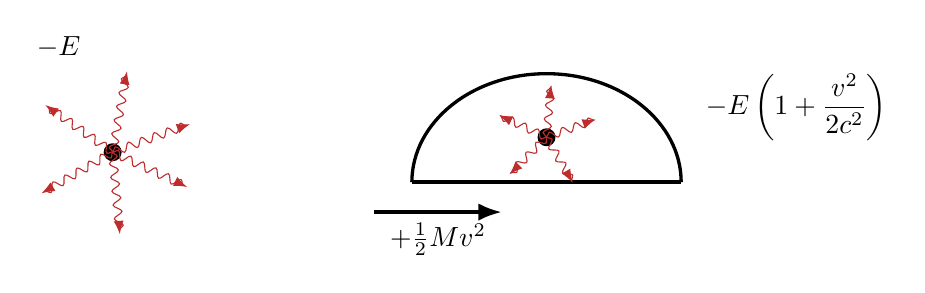
\begin{tikzpicture}[>=Latex,x=0.95cm,y=0.95cm]
  % left isotropic radiator
  \fill[black] (-3.8,0.3) circle (0.12);
  \foreach \a in {20,80,145,210,275,335}
    \draw[inkred,decorate,decoration={snake,amplitude=1.5pt,segment length=5pt},->]
      (-3.8,0.3)--++(\a:1.1);
  \node[left] at (-4.1,1.7) {$-E$};

  % moving dome
  \draw[very thick] (0.2,-0.1) arc (180:0:1.8 and 1.45);
  \draw[very thick] (0.2,-0.1)--(3.8,-0.1);
  \draw[->,very thick] (-0.3,-0.5)--(1.4,-0.5)
    node[midway,below] {$+\tfrac12 Mv^2$};
  \fill[black] (2.0,0.5) circle (0.12);
  \foreach \a in {20,85,155,225,300}
    \draw[inkred,decorate,decoration={snake,amplitude=1.4pt,segment length=5pt},->]
      (2.0,0.5)--++(\a:0.7);
  \node[right,align=left] at (4.0,0.9)
    {$-E\left(1+\dfrac{v^2}{2c^2}\right)$};
\end{tikzpicture}
\end{center}

De onderste energiebalans staat genoteerd als:

$$
-E+\frac12 m v^2
=
\frac12 M v^2
-
E\left(1+\frac{v^2}{c^2}\right).
$$

Ten slotte:

\begin{align*}
\frac{E}{c^2}&=m_1-m_2,\\
&\Longrightarrow E=mc^2.
\end{align*}

\noindent
De factoren $\tfrac{1}{2}$ in de Dopplerbenadering zijn niet overal
consistent in de handgeschreven pagina; bovenstaande vergelijkingen volgen
de afzonderlijke notities letterlijk.

% --------------------------------------------------------------------------
\newpage
\section*{PDF-pagina 10 --- de vijf staten van een stof}

De titel luidt letterlijk ``De 5 Staten van een stof''. De pagina ordent vijf
toestanden van koud naar heet.

\begin{center}
\begin{tabularx}{\textwidth}{>{\bfseries}l>{\raggedright\arraybackslash}Xl}
\toprule
\textbf{Toestand} & \textbf{Letterlijke of bijna-letterlijke notitie} &
\textbf{Temperatuur}\\
\midrule
Vast &
IJs; atomen blijven op hun positie. De kern kan nog wel in het atoom bewegen. &
koud\\
Vloeibaar &
Water kan van vorm veranderen, maar ``atoom zoekt zichzelf op''.
\uncertain{formulering} &
gemiddeld\\
Gas &
Damp; de atomen botsen door de hitte van elkaar af. &
heet\\
Bose-Einsteincondensaat &
De kernen blijven op positie, waardoor de elektronen
\uncertain{``in harmonie veranderen in één golf''}. Een B.E.C. kan men
\uncertain{``op één plek teleportatie uitvoeren''}. &
extreem koud\\
Plasma &
De kernen trillen zo hard dat de protonen, neutronen en elektronen
één geheel ``lava'' worden. &
extreem heet\\
\bottomrule
\end{tabularx}
\end{center}

Bij het Bose-Einsteincondensaat staat daarnaast ``extreem vast'' geschreven.
De formulering over teleportatie en de beschrijving van plasma zijn
letterlijk overgenomen en niet natuurkundig gecorrigeerd.

\begin{center}
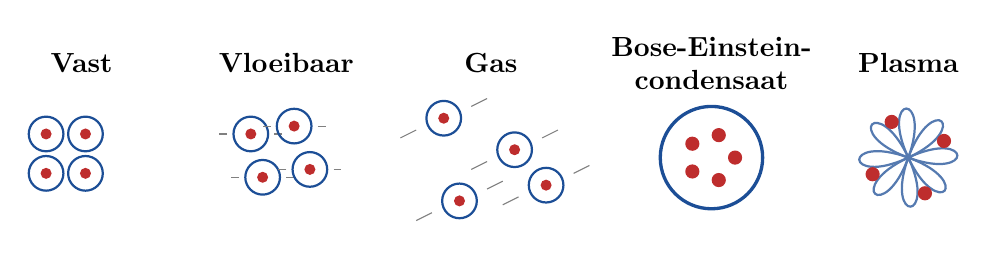
\begin{tikzpicture}[x=1cm,y=1cm]
  % solid
  \node[font=\bfseries] at (-4.7,2.1) {Vast};
  \foreach \x/\y in {-5.15/1.2,-4.65/1.2,-5.15/0.7,-4.65/0.7}
  {
    \draw[inkblue,thick] (\x,\y) circle (0.22);
    \fill[inkred] (\x,\y) circle (0.07);
  }

  % liquid
  \node[font=\bfseries] at (-2.1,2.1) {Vloeibaar};
  \foreach \x/\y in {-2.55/1.2,-2.0/1.3,-2.4/0.65,-1.8/0.75}
  {
    \draw[inkblue,thick] (\x,\y) circle (0.22);
    \fill[inkred] (\x,\y) circle (0.07);
    \draw[black!50] (\x-0.3,\y)--(\x-0.4,\y);
    \draw[black!50] (\x+0.3,\y)--(\x+0.4,\y);
  }

  % gas
  \node[font=\bfseries] at (0.5,2.1) {Gas};
  \foreach \x/\y in {-0.1/1.4,0.8/1.0,0.1/0.35,1.2/0.55}
  {
    \draw[inkblue,thick] (\x,\y) circle (0.22);
    \fill[inkred] (\x,\y) circle (0.07);
    \draw[black!50] (\x-0.35,\y-0.15)--(\x-0.55,\y-0.25);
    \draw[black!50] (\x+0.35,\y+0.15)--(\x+0.55,\y+0.25);
  }

  % BEC
  \node[font=\bfseries,align=center] at (3.3,2.1) {Bose-Einstein-\\condensaat};
  \draw[inkblue,very thick] (3.3,0.9) circle (0.65);
  \foreach \a in {0,72,...,288}
    \fill[inkred] ({3.3+0.3*cos(\a)},{0.9+0.3*sin(\a)}) circle (0.09);

  % Plasma
  \node[font=\bfseries] at (5.8,2.1) {Plasma};
  \foreach \a in {0,45,...,315}
    \draw[inkblue!75,thick] (5.8,0.9)
       .. controls ({5.8+0.9*cos(\a+25)},{0.9+0.9*sin(\a+25)})
       and ({5.8+0.9*cos(\a-20)},{0.9+0.9*sin(\a-20)})
       .. cycle;
  \foreach \a in {25,115,205,295}
    \fill[inkred] ({5.8+0.5*cos(\a)},{0.9+0.5*sin(\a)}) circle (0.09);
\end{tikzpicture}
\end{center}

\end{document}
